\documentclass[a4paper]{article}

\usepackage{amsmath}
\usepackage{amssymb}
\usepackage{amsfonts}
\usepackage[style=iso]{datetime2}
\usepackage[explicit]{titlesec}
\usepackage{amsthm}
\usepackage{mathrsfs}
\usepackage{array}
\usepackage{graphicx}
\usepackage{mathtools} % Provides \mathrlap command
\usepackage{float}
\usepackage[skip=1em,indent]{parskip}
\usepackage{caption}
\usepackage{hyperref}
\usepackage{tocloft}
\usepackage{mathtools}

\usepackage{tikz}
\tikzset{>=latex} % for LaTeX arrow head
\usepackage{pgfplots} % for the axis environment
\usetikzlibrary{calc,decorations.markings}

\pgfplotsset{compat=1.18, every tick label/.append style={font=\footnotesize}}

\graphicspath{ {./Images/} }

\makeatletter
\def\th@plain{%
  \thm@notefont{}% same as heading font
  \itshape % body font
}
\def\th@definition{%
  \thm@notefont{}% same as heading font
  \normalfont % body font
}
\makeatother

\newcommand*\diff{\mathop{}\!d} % for the differential in integrals

\NewCommandCopy{\oldIm}{\Im}
\renewcommand{\Im}{\mathop{\oldIm\mathfrak{m}}}
\NewCommandCopy{\oldRe}{\Re}
\renewcommand{\Re}{\mathop{\oldRe\mathfrak{e}}}

\newtheorem{theorem}{Theorem}
\newtheorem{lemma}[theorem]{Lemma}
\newtheorem{proposition}[theorem]{Proposition}
\newtheorem{corollary}{Corollary}[theorem]

\theoremstyle{definition}
\newtheorem{definition}{Definition}

% \setlength{\cftsecnumwidth}{3em}

\begin{titlepage}
\title{The Dirichlet Integral}
\author{Abdul Musthakin}
\date{\today}
\end{titlepage}

% \renewcommand{\thesection}{\Roman{section}}

\allowdisplaybreaks

\setlength{\parindent}{0pt}

\begin{document}
\maketitle

\begin{figure}[!h]
    \centering
    \scalebox{1.7}{
        \begin{tikzpicture}
            \begin{axis}[
                    clip=false,
                    xmin=-4.5*pi,xmax=4.5*pi,
                    yscale=0.75,
                    axis lines=middle,
                    xlabel= $x$,
                    xlabel style={at={(1,0.35)}},
                    ylabel=$y$,
                    ymin=-0.5,ymax=1.5,
                    xtick={-4*pi, -3*pi,-2*pi,-pi,0,pi,2*pi,3*pi, 4*pi},
                    xticklabels={$-4\pi$,$-3\pi$,$-2\pi$, $-\pi$, $0$,$\pi$,$2\pi$, $3\pi$, $4\pi$},
                    xticklabel style={anchor=north},
                    ytick={1},
                    yticklabels={$1$},
                ]
                \addplot[domain=-4*pi:4*pi,samples=200,red]{sin(deg(x))/x};
            \end{axis}
        \end{tikzpicture}}
    \captionsetup{justification=centering}
    \caption{$y = \frac{\sin x}{x}$}
    \label{fig:fig1}
\end{figure}

\pagebreak

\tableofcontents

\section{Introduction}

The Dirichlet integral, which I will denote with $\mathcal{I}$, is a pretty well-known integral with quite a few ways to evaluate it.
I will attempt to outline as many of those ways as possible.
Below is $\mathcal{I}$ and the value we claim it has.
\begin{equation}
    \mathcal{I} \coloneq \int_{-\infty}^{\infty} \frac{\sin x}{x} \diff x = \pi
\end{equation}
Firstly, whilst some sources may refer to the integral with limits 0 and $\infty$ as the Dirichlet integral, I will refer to the one above.
Due to the fact that the integrand is an even function, it is clear that these two integrals differ by a factor of 2.
This is a result that is pretty important, and one that we will use to evaluate $\mathcal{I}$.

The integrand is undefined at $x=0$.
However, this will not be a problem when we try to integrate it, as the discontinuity is removable.
The limit of the integrand as $x \to 0$ exists and is equal to 1; it is one of the most famous limits.
Besides $x=0$, the integrand is defined everywhere.

\section{Convergence}

Before we actually evaluate the Dirichlet integral, we should show that it actually converges.
It turns out $\mathcal{I}$ does converge, but only conditionally.
\begin{proposition} \label{thm:convergence proposition 1}
    The integral
    \begin{equation*}
        \mathcal{I} \coloneq \int_{-\infty}^{\infty} \frac{\sin x}{x} \diff x
    \end{equation*}
    converges.
\end{proposition}
\begin{proof}
    Let
    \begin{equation*}
        a_k \coloneq \int_{\pi k}^{\pi(k+1)} \frac{\sin x}{x} \diff x,
    \end{equation*}
    where $k \in \mathbb{Z}_{\geq 0}$.
    Then,
    \begin{equation*}
        |a_k| = \int_{\pi k}^{\pi(k+1)} \left| \frac{\sin x}{x} \right| \diff x = \int_{\pi k}^{\pi(k+1)} \frac{|\sin x|}{x} \diff x.
    \end{equation*}
    Notice that $\lim_{k \to \infty} |a_k| = 0$, since (as $k \to \infty$)
    \begin{align*}
        \int_{\pi k}^{\pi(k+1)} \frac{|\sin x|}{x} \diff x & \leq \int_{\pi k}^{\pi(k+1)} \frac{\diff x}{x} & \qquad \qquad \because 0 \leq |\sin x| \leq 1 \\
                                                           & = \ln \left(\frac{k+1}{k}\right) \to 0.        &
    \end{align*}
    Also note that
    \begin{align*}
        \int_{0}^{t} \frac{\sin x}{x} \diff x                                     & = \int_{0}^{\pi k} \frac{\sin x}{x} \diff x + \int_{\pi k}^{t} \frac{\sin x}{x} \diff x \\
        \leadsto \quad \lim_{\substack{t \to \infty                                                                                                                         \\ k \to \infty}} \int_{0}^{t} \frac{\sin x}{x} \diff x &= \lim_{\substack{t \to \infty \\ k \to \infty}} \left( \int_{0}^{\pi k} \frac{\sin x}{x} \diff x + \int_{\pi k}^{t} \frac{\sin x}{x} \diff x  \right) \\
        \leadsto \quad \lim_{t \to \infty}  \int_{0}^{t} \frac{\sin x}{x} \diff x & = \lim_{k \to \infty}\int_{0}^{\pi k} \frac{\sin x}{x} \diff x                          \\
        \leadsto \quad \lim_{t \to \infty}  \int_{0}^{t} \frac{\sin x}{x} \diff x & = \lim_{t \to \infty}\int_{0}^{\pi t} \frac{\sin x}{x} \diff x,
    \end{align*}
    since (in the limits considered)
    \begin{align*}
        \left|\int_{\pi k}^{t} \frac{\sin x}{x} \diff x \right| & \leq \int_{\pi k}^{t} \frac{|\sin x|}{x} \diff x \\
                                                                & \leq \int_{\pi k}^{t} \frac{\diff x}{x}          \\
                                                                & = \ln \left(\frac{t}{\pi k}\right) \to 0         \\
        \leadsto   \quad                                        & \int_{\pi k}^{t} \frac{\sin x}{x} \diff x \to 0.
    \end{align*}
    Hence,
    \begin{align*}
        \int_{0}^{\pi t} \frac{\sin x}{x} \diff x                 & = \sum_{k=0}^{t-1} a_k     \\
        \leadsto \quad \int_{0}^{\infty} \frac{\sin x}{x} \diff x & = \sum_{k=0}^{\infty} a_k.
    \end{align*}
    Now, consider the statement $|a_{+1}| < |a_k|$ for all $k$.
    We can show that this is true using the fact that $|\sin (\pi (k+1) + t)| = |\sin(\pi k + t)|$ for all $t$, and thus
    \begin{equation*}
        \frac{|\sin (\pi (k+1) + t)|}{\pi(k+1) + t} < \frac{|\sin (\pi k + t)|}{\pi k + t}.
    \end{equation*}
    Therefore,
    \begin{align*}
        |a_{k+1}| & = \int_{\pi (k+1)}^{\pi(k+2)} \frac{|\sin x|}{x} \diff x              \\
                  & = \int_{0}^{\pi} \frac{|\sin (\pi (k+1) + t)|}{\pi (k+1) + t} \diff x \\
                  & < \int_{0}^{\pi} \frac{|\sin (\pi k + t)|}{\pi k + t} \diff x         \\
                  & = \int_{\pi k}^{\pi(k+1)} \frac{\sin x}{x} \diff x, \text{where } k   \\
                  & = |a_k|.
    \end{align*}
    Additionally, from Figure~\ref{fig:fig1}, it can be seen that is positive for even $k$ and negative for odd $k$.
    Via the alternating series test, it follows that
    \begin{equation*}
        \sum_{k=0}^{\infty} a_k
    \end{equation*}
    converges, and therefore
    \begin{equation*}
        \int_{0}^{\infty} \frac{\sin x}{x} \diff x
    \end{equation*}
    also converges.
    As the integrand is an even function, $\mathcal{I}$ converges and evaluates to twice the above integral.
\end{proof}
\begin{proposition} \label{thm:convergence proposition 2}
    The integral
    \begin{equation*}
        \int_{-\infty}^{\infty} \frac{|\sin x|}{x} \diff x
    \end{equation*}
    diverges.
\end{proposition}
\begin{proof}
    It suffices to show that
    \begin{equation*}
        \int_{0}^{\infty} \frac{|\sin x|}{x} \diff x
    \end{equation*}
    diverges, for which it suffices to show that
    \begin{equation*}
        \sum_{k=0}^{\infty} |a_k|
    \end{equation*}
    diverges.
    To do this, we will use the fact that
    \begin{equation*}
        \frac{1}{x} \geq \frac{1}{\pi(k+1)}
    \end{equation*}
    for all $x \in [\pi k, \pi(k+1)]$.
    This allows us to obtain a lower bound for $|a_k|$.
    \begin{align*}
        |a_k| & = \int_{\pi k}^{\pi(k+1)} \frac{|\sin x|}{x} \diff x                       \\
              & \geq \int_{\pi k}^{\pi(k+1)} \frac{|\sin x|}{\pi(k+1)} \diff x             \\
              & = \frac{1}{\pi(k+1)} \int_{\pi k}^{\pi(k+1)} |\sin x| \diff x              \\
              & = \frac{1}{\pi(k+1)} \left| \int_{\pi k}^{\pi(k+1)} \sin x \diff x \right| \\
              & = \frac{2}{\pi(k+1)}
    \end{align*}
    Hence,
    \begin{equation*}
        \sum_{k=0}^{\infty} |a_k| \geq \frac{2}{\pi} \sum_{k=0}^{\infty} \frac{1}{k+1},
    \end{equation*}
    which diverges.
\end{proof}

\section{Laplace Transform}

\begin{definition}[Laplace Transform]
    Let $f: \mathbb{R}_{>0} \to \mathbb{R}$ be a function of $t$.
    The Laplace transform of $f$, denoted $\mathscr{L}\{f\}$, is a function of $s \in \mathbb{C}$ defined by
    \begin{equation}
        \mathscr{L} \{f(t)\}(s) \coloneq \int_{0}^{\infty} e^{-st} f(t) \diff t \coloneq \lim_{\varepsilon \to 0^+} \int_{\varepsilon}^{\infty} e^{-st} f(t) \diff t,
    \end{equation}
    if the integral converges.
    Note that this is specifically the definition of the Laplace transform of a function with a discontinuity at $x=0$, as that is what we are working with.
\end{definition}
Now, let us derive a property of the Laplace transform that we will use to evaluate the Dirichlet Integral.
\begin{proposition} \label{thm:Laplace property proposition}
    If
    \begin{equation*}
        \int_{0}^{\infty} \frac{|f(t)|}{t} e^{-st} \diff t
    \end{equation*}
    converges, then
    \begin{equation}
        \mathscr{L} \left\{\frac{f(t)}{t}\right\}(s) = \int_{s}^{\infty} \mathscr{L}\{f(t)\}(\varphi) \diff \varphi.
    \end{equation}
\end{proposition}
\begin{proof}
    We can write
    \begin{equation*}
        \int_{0}^{\infty} \frac{|f(t)|}{t} e^{-st} \diff t = \int_{0}^{\infty} \int_{s}^{\infty} e^{-\varphi t} |f(t)| \diff \varphi \diff t.
    \end{equation*}
    The absolute convergence of the double integral justifies swapping the order of integration by Fubini's theorem.
    Thus,
    \begin{align*}
        \mathscr{L} \left\{\frac{f(t)}{t}\right\}(s) & = \int_{0}^{\infty} \frac{f(t)}{t} e^{-st} \diff t                              \\
                                                     & = \int_{0}^{\infty} \int_{s}^{\infty} e^{-\varphi t} f(t) \diff \varphi \diff t \\
                                                     & = \int_{s}^{\infty} \int_{0}^{\infty} e^{-\varphi t} f(t) \diff t \diff \varphi \\
                                                     & = \int_{s}^{\infty} \mathscr{L}\{f(t)\}(\varphi) \diff \varphi.
    \end{align*}
\end{proof}
It would make sense to first show that the condition for Proposition~\ref{thm:Laplace property proposition}.
That is, we need to show that
\begin{equation*}
    \mathscr{L} \left\{\left|\frac{\sin t}{t}\right|\right\}(s) = \int_{0}^{\infty} \frac{|\sin t|}{t} e^{-st} \diff t
\end{equation*}
converges, which is pretty easy to do via the comparison test.
By the mean value theorem, there exists $\xi \in \mathbb{R}_{>0}$ such that
\begin{alignat*}{4}
     &                & \frac{\sin t - \sin 0}{t - 0} & = \cos \xi   &                                       \\
     & \leadsto \quad & \sin t                        & = t \cos \xi &                                       \\
     &                &                               & \leq t       & \qquad\qquad \because \cos \xi \leq 1
\end{alignat*}
for $t>0$.
Therefore,
\begin{alignat*}{3}
     &                & \frac{\sin t}{t}                                     & \leq 1                                                \\
     & \leadsto \quad & \frac{|\sin t|}{t}                                   & \leq 1                                                \\
     & \leadsto\quad  & \frac{|\sin t|}{t} e^{-st}                           & \leq e^{-st}                                          \\
     & \leadsto \quad & \int_{0}^{\infty} \frac{|\sin t|}{t} e^{-st} \diff t & \leq \int_{0}^{\infty} e^{-st} \diff t = \frac{1}{s}.
\end{alignat*}
for $s>0$.
Now we will evaluate the Laplace transform of $f(t) = \sin t$ first, which involves standard integration by parts.
\begin{alignat*}{3}
     &                & \mathscr{L}\{\sin t\}(s)                                & = \int_{0}^{\infty} e^{-st}\sin t \diff t                                                                                       \\
     &                &                                                         & = \left. - \frac{1}{s} e^{-st} \sin t \right|_{t\to 0}^{t\to \infty} + \frac{1}{s} \int_{0}^{\infty} e^{-st} \cos t \diff t     \\
     &                &                                                         & = \frac{1}{s} \int_{0}^{\infty} e^{-st} \cos t \diff t                                                                          \\
     &                &                                                         & = \left. - \frac{1}{s^2} e^{-st} \cos t \right|_{t\to 0}^{t\to \infty} - \frac{1}{s^2} \int_{0}^{\infty} e^{-st} \sin t \diff t \\
     &                &                                                         & =  \frac{1}{s^2} - \frac{1}{s^2} \mathscr{L}\{\sin t\}(s)                                                                       \\
     & \leadsto \quad & \mathscr{L}\{\sin t\}(s) \left(1 + \frac{1}{s^2}\right) & = \frac{1}{s^2}                                                                                                                 \\
     & \leadsto\quad  & \mathscr{L}\{\sin t\}(s)                                & = \frac{\frac{1}{s^2}}{1 + \frac{1}{s^2}}                                                                                       \\
     &                &                                                         & = \frac{1}{s^2 + 1}
\end{alignat*}
We can evaluate $\mathcal{I}$ rather easily with these results.
\begin{align*}
    \mathcal{I} & = 2\int_{0}^{\infty} \frac{\sin x}{x} \diff x                                                         \\
                & = 2 \int_{0}^{\infty} \lim_{s \to 0}\frac{\sin x}{x} e^{-sx} \diff x                                  \\
                & = 2 \lim_{s \to 0} \int_{0}^{\infty} \frac{\sin x}{x} e^{-sx} \diff x                                 \\
                & = 2 \lim_{s \to 0} \mathscr{L} \left\{\frac{\sin x}{x}\right\}(s)                                     \\
                & = 2 \lim_{s \to 0} \int_{s}^{\infty} \mathscr{L} \left\{\sin x\right\}(\varphi) \diff \varphi         \\
                & = 2 \lim_{s \to 0} \int_{s}^{\infty} \frac{\diff \varphi}{\varphi^2 + 1}                              \\
                & = 2 \lim_{s \to 0} \left.\vphantom{\int} \arctan \varphi \right|_{\varphi \to s}^{\varphi \to \infty} \\
                & = 2 \lim_{s \to 0} \left[\frac{\pi}{2} - \arctan s \right]                                            \\
                & = 2 \cdot \frac{\pi}{2}                                                                               \\
                & = \pi
\end{align*}
Whilst this was a "simple" evaluation, there is a caveat.
We interchanged a limit and an integral, which we can show to be valid via the final value theorem for Laplace transforms.
\begin{proposition} \label{thm:FVT proposition}
    \begin{equation*}
        \lim_{s \to 0} \int_{0}^{\infty} \frac{\sin x}{x} e^{-sx} \diff x = \int_{0}^{\infty} \lim_{s \to 0}\frac{\sin x}{x} e^{-sx} \diff x
    \end{equation*}
\end{proposition}
\begin{proof}
    Let $h: \mathbb{R}_{>0} \to \mathbb{R}$, where
    \begin{equation*}
        h(t) \coloneq \frac{\sin t}{t}.
    \end{equation*}
    Let
    \begin{equation*}
        f(x) \coloneq \int_{0}^{x} h(t) \diff t,
    \end{equation*}
    which converges for $x \to \infty$ by Proposition~\ref{thm:convergence proposition 1}.
    Note that $f'(t) = h(t)$.
    Consider the following application of integration by parts: for $s>0$,
    \begin{align*}
        s \int_{0}^{\infty} e^{-st} f(t) \diff t & = -e^{-st} f(t) \bigg|_{t\to 0}^{t\to \infty} + \int_{0}^{\infty} e^{-st} f'(t) \diff t \\
                                                 & = f(0) + \int_{0}^{\infty} e^{-st} h(t) \diff t                                         \\
                                                 & = \int_{0}^{\infty} e^{-st} h(t) \diff t.
    \end{align*}
    By the final value theorem, the LHS converges to $\lim_{x \to \infty} f(x)$ as $s \to 0$.
    Hence,
    \begin{equation*}
        \lim_{s\to 0} \int_{0}^{\infty} \frac{\sin x}{x} e^{-sx} \diff x = \int_{0}^{\infty} \frac{\sin x}{x} \diff x = \int_{0}^{\infty} \lim_{s \to 0} \frac{\sin x}{x} e^{-sx} \diff x.
    \end{equation*}
\end{proof}

\section{Double Integration}

The first method relied on a property of the Laplace transform, which itself relied on the ability to change the order of a double integral.
We can strip away a lot of the set-up by immediately turning our problem into one of double integration.
\begin{align*}
    \mathcal{I} & = \int_{-\infty}^{\infty} \frac{\sin x}{x} \diff x                                  \\
                & = 2\int_{0}^{\infty} \frac{\sin x}{x} \diff x                                       \\
                & = 2\int_{0}^{\infty} \int_{0}^{\infty} e^{-\varphi x} \sin x  \diff \varphi \diff x \\
                & = 2\int_{0}^{\infty} \int_{0}^{\infty} e^{-\varphi x} \sin x  \diff x \diff \varphi \\
                & = 2\int_{0}^{\infty} \frac{\diff \varphi}{\varphi^2 + 1}                            \\
                & = \pi
\end{align*}
The way we have done things here appears to omit the problem regarding limits and integrals which was previously resolved by Proposition~\ref{thm:FVT proposition}.
However, it has simply been translated into a problem regarding swapping the order of integration.
Fubini's theorem no longer justifies it due to the integral not being absolutely convergent.
\begin{equation*}
    \int_{0}^{\infty} \int_{0}^{\infty} e^{-\varphi x} | \sin x | \diff \varphi \diff x = \int_{0}^{\infty} \frac{|\sin x|}{x} \diff x,
\end{equation*}
which is divergent by Proposition~\ref{thm:convergence proposition 2}.
This could be resolved by rewriting the integral as the limit of a Laplace transform as we have done before.
However, there is an alternative method as I will illustrate.
\begin{theorem}[Weierstrass M-test for Integrals] \label{thm:Weierstrass M-test}
    Suppose $M(x)$ is nonnegative on $[a,b)$,
    \begin{equation*}
        \int_{a}^{b} M(x)
    \end{equation*}
    converges, and $|f(x,y)| \leq M(x)$ for all $y \in S$ and for all $x \in [a,b)$.
    Then,
    \begin{equation*}
        \int_{a}^{b} f(x,y) \diff x
    \end{equation*}
    converges absolutely uniformly on S.
\end{theorem}
\begin{proposition} \label{thm:double integral proposition}
    \begin{equation*}
        \int_{0}^{\infty} \int_{0}^{\infty} e^{-\varphi x} \sin x \diff x \diff \varphi = \int_{0}^{\infty} \int_{0}^{\infty} e^{-\varphi x} \sin x  \diff \varphi \diff x
    \end{equation*}
\end{proposition}
\begin{proof}
    Since the integrand is continuous, Fubini's theorem permits changing the order of intergration on the bounded rectangle
    \begin{equation*}
        \int_{a}^{b} \int_{c}^{d} e^{-\varphi x} \sin x \diff x \diff \varphi = \int_{c}^{d} \int_{a}^{b} e^{-\varphi x} \sin x  \diff \varphi \diff x,
    \end{equation*}
    where $0 < a < b$ and $0 < c < d$.
    The inner integral on the RHS can be shown to be uniformly convergent for $x \in [c,d]$ via applying the Weierstrass M-test as $a \to 0$ and $b \to \infty$.
    Note that
    \begin{equation*}
        \left|e^{-\varphi x} \sin x \right| = e^{-\varphi x} |\sin x| \leq e^{-\varphi x} \leq e^{-\varphi c}.
    \end{equation*}
    It is true that $e^{-\varphi c}$ is nonnegative on $[a,b)$ and
    \begin{equation*}
        \int_{0}^{\infty} e^{-\varphi c} \diff \varphi = \frac{1}{c}
    \end{equation*}
    converges for all $c>0$.
    All the conditions of the Weierstrass M-test have been satisfied and uniform convergence for $x \in [c,d]$ is shown by Theorem~\ref{thm:Weierstrass M-test}.
    It thus follows that we may pass the limits under the RHS integral.
    \begin{align*}
        \int_{0}^{\infty} \int_{c}^{d} e^{-\varphi x} \sin x \diff x \diff \varphi & = \lim_{\substack{a \to 0                                                     \\ b \to \infty}} \int_{c}^{d} \int_{a}^{b} e^{-\varphi x} \sin x  \diff \varphi \diff x \\
                                                                                   & = \int_{c}^{d} \lim_{\substack{a \to 0                                        \\ b \to \infty}} \int_{a}^{b} e^{-\varphi x} \sin x  \diff \varphi \diff x \\
                                                                                   & = \int_{c}^{d} \int_{0}^{\infty} e^{-\varphi x} \sin x  \diff \varphi \diff x
    \end{align*}
    We wish to do the same for the LHS integral with the limits $c \to 0$ and $d \to \infty$.
    We know that the inner integral converges pointwise to the Laplace transform of $\sin x$.
    Also, note that (using integration by parts)
    \begin{align*}
        \left|\int_{c}^{d} e^{-\varphi x} \sin x \diff x \right| & = \left| \frac{-e^{-\varphi x} (\varphi\sin x + \cos x)}{1+\varphi^2} \right|_{x= c}^{x = d}                                  \\
                                                                 & \leq \left|\frac{e^{-\varphi c} \cos c}{1+\varphi^2}\right| + \left|\frac{\varphi e^{ -\varphi c} \sin c}{1+\varphi^2}\right| \\
                                                                 & + \left|\frac{e^{-\varphi d} \cos d}{1+\varphi^2}\right| + \left|\frac{\varphi e^{-\varphi d} \sin d}{1+\varphi^2}\right|     \\
                                                                 & \leq \frac{A}{1+\varphi^2},
    \end{align*}
    where A is a constant.
    This bound holds because
    \begin{equation*}
        \left| \frac{e^{-\varphi x} \cos x}{1+\varphi^2}\right| = \frac{e^{-\varphi x}|\cos x|}{1 +\varphi^2} \leq \frac{1}{1+\varphi^2},
    \end{equation*}
    and $f(x) = \varphi e^{-\varphi x} \sin x$ has a maximum for $x \in [0,\infty)$ at $x^* = \arctan \left(\frac{1}{\varphi}\right)$, where
    \begin{equation*}
        f(x^*) = \varphi e^{-\varphi \arctan\left(\frac{1}{\varphi}\right)} \sin \left(\arctan\left(\frac{1}{\varphi}\right)\right) = \varphi e^{-\varphi \arctan\left(\frac{1}{\varphi}\right)}\frac {1}{\varphi \sqrt{1 + \left(\frac{1}{\varphi}\right)^2}} \leq 1.
    \end{equation*}
    We now have a function that dominates the integral, and it can be shown that it is (Lebesgue) integrable on $(0, \infty)$:
    \begin{equation*}
        \int_{0}^{\infty} \left|\frac{1}{\varphi^2 + 1}\right| \diff \varphi = \int_{0}^{\infty} \frac{1}{\varphi^2 + 1} \diff \varphi = \frac{\pi}{2}.
    \end{equation*}
    Let $(c_n) \to 0$ and $(d_n) \to \infty$ be arbitrary.
    Then,
    \begin{equation*}
        \lim_{\substack{c \to 0 \\ d\to \infty}} \int_{c}^{d} e^{-\varphi x} \sin x  \diff \varphi \diff x = \lim_{n \to \infty}  \int_{c_n}^{d_n} e^{-\varphi x} \sin x  \diff \varphi \diff x.
    \end{equation*}
    We can now apply the dominated convergence theorem (DCT).
    Therefore,
    \begin{align*}
        \int_{0}^{\infty} \int_{0}^{\infty} e^{-\varphi x} \sin x  \diff \varphi \diff x & = \lim_{\substack{c \to 0                                                                             \\ d \to \infty}}\int_{0}^{\infty} \int_{c}^{d} e^{-\varphi x} \sin x \diff x \diff \varphi \\
                                                                                         & = \lim_{n \to \infty} \int_{0}^{\infty} \int_{c_n}^{d_n} e^{-\varphi x} \sin x  \diff x \diff \varphi \\
                                                                                         & = \int_{0}^{\infty} \lim_{n \to \infty} \int_{c_n}^{d} e^{-\varphi x} \sin x  \diff x \diff \varphi   \\
                                                                                         & =\int_{0}^{\infty} \int_{0}^{\infty} e^{-\varphi x} \sin x  \diff x \diff \varphi.
    \end{align*}
\end{proof}

\section{Differentiation under the Integral Sign}

This method is similar to the previous two.
We will use differentiation under the integral sign, also known as the Leibniz rule or Feynman's trick.
We want to first parameterise the integral in terms of the variable $\alpha$.
Let
\begin{equation*}
    \mathcal{I}(\alpha) \coloneq \int_{0}^{\infty} \frac{\sin x}{x} e^{- \alpha x} \diff x,
\end{equation*}
where $\alpha > 0$ (we have previously shown that this converges for these values of $\alpha$).
This means that our target integral is given by
\begin{equation*}
    \mathcal{I} \coloneq \int_{-\infty}^{\infty} \frac{\sin x}{x} \diff x = 2\mathcal{I}(0).
\end{equation*}
The derivative of the integrand with respect to $\alpha$ is
\begin{equation*}
    \frac{\partial}{\partial \alpha} \frac{\sin x}{x} e^{- \alpha x} = - e^{- \alpha x} \sin x.
\end{equation*}
The integral of this, as $a \to 0$ and $b \to \infty$,
uniformly converges for all $\alpha \in [c,d] \subset (0, \infty)$ by \hyperref[thm:Weierstrass M-test]{Theorem~\ref*{thm:Weierstrass M-test} (\nameref*{thm:Weierstrass M-test})} via the same logic as that used in the proof of Proposition~\ref{thm:double integral proposition}; this justifies differentiating under the integral sign.
Then,
\begin{align*}
    \frac{d\mathcal{I}}{d \alpha} & = \frac{d}{d \alpha} \int_{0}^{\infty} \frac{\sin x}{x} e^{- \alpha x} \diff x               \\
                                  & = \int_{0}^{\infty} \frac{\partial}{\partial \alpha} \frac{\sin x}{x} e^{- \alpha x} \diff x \\
                                  & = - \int_{0}^{\infty} e^{- \alpha x} \sin x  \diff x                                         \\
                                  & = - \mathscr{L} \{\sin x\}(\alpha)                                                           \\
                                  & = - \frac{1}{\alpha^2 + 1}.
\end{align*}
Integrating with respect to $\alpha$ gives
\begin{equation*}
    \mathcal{I}(\alpha) = - \int \frac{\diff \alpha}{\alpha^2 + 1} = C - \arctan \alpha
\end{equation*}
We have to evaluate the constant of integration.
In this particular case, we take the limit of $\mathcal{I}(\alpha)$ as $\alpha \to \infty$.
\begin{alignat*}{3}
     &                & \lim_{\alpha \to \infty} \int_{0}^{\infty} \frac{\sin x}{x} e^{- \alpha x} \diff x & =  \lim_{\alpha \to \infty} \left[C - \arctan \alpha\right] \\
     & \leadsto \quad & \int_{0}^{\infty} \lim_{\alpha \to \infty} \frac{\sin x}{x} e^{- \alpha x} \diff x & = C - \lim_{\alpha \to \infty} \arctan \alpha               \\
     & \leadsto \quad & \int_{0}^{\infty} 0 \diff x                                                        & = C - \frac{\pi}{2}                                         \\
     & \leadsto \quad & 0                                                                                  & = C - \frac{\pi}{2}                                         \\
     & \leadsto \quad & C                                                                                  & = \frac{\pi}{2}
\end{alignat*}
Therefore,
\begin{equation*}
    \mathcal{I}(\alpha) = \frac{\pi}{2} - \arctan \alpha.
\end{equation*}
Finally,
\begin{align*}
    \mathcal{I} & = 2\mathcal{I}(0)                          \\
                & = 2 \left(\frac{\pi}{2} - \arctan 0\right) \\
                & = 2 \cdot \frac{\pi}{2}                    \\
                & = \pi.
\end{align*}
To justify swapping the limit and integral above, we can use the initial value theorem for Laplace transforms.
\begin{proposition} \label{thm:IVT proposition}
    \begin{equation*}
        \lim_{\alpha \to \infty} \int_{0}^{\infty} \frac{\sin x}{x} e^{- \alpha x} \diff x = \int_{0}^{\infty} \lim_{\alpha \to \infty} \frac{\sin x}{x} e^{- \alpha x} \diff x
    \end{equation*}
\end{proposition}
\begin{proof}
    Consider the proof of Proposition~\ref{thm:FVT proposition}, including its definitions of $h$ and $f$.
    Then, for $\alpha>0$, we have
    \begin{equation*}
        \alpha \int_{0}^{\infty} e^{-\alpha t} f(t) \diff t = \int_{0}^{\infty} e^{-\alpha t} h(t) \diff t.
    \end{equation*}
    By the initial value theorem, the LHS converges to $\lim_{x \to 0} f(x) = 0$ as $\alpha \to \infty$.
    Hence,
    \begin{equation*}
        \lim_{\alpha\to \infty} \int_{0}^{\infty} \frac{\sin x}{x} e^{-sx} \diff x = 0 = \int_{0}^{\infty} \lim_{\alpha \to \infty} \frac{\sin x}{x} e^{-sx} \diff x.
    \end{equation*}
\end{proof}

\section{Contour Integration}

Let $f: \mathbb{C} \setminus \{0\} \to \mathbb{C}$ be defined by
\begin{equation*}
    f(z) \coloneq \frac{e^{iz}}{z}.
\end{equation*}
By Euler's formula, for $x \in \mathbb{R}$,
\begin{equation*}
    \Im (f(x)) = \frac{\sin x}{x}.
\end{equation*}
However, note that
\begin{equation*}
    \mathcal{I} \coloneq \int_{-\infty}^{\infty} \frac{\sin x}{x} \diff x \neq \Im \left( \int_{-\infty}^{\infty} \frac{e^{iz}}{z} \diff z \right),
\end{equation*}
as the latter integral does not converge due to the singularity at $z=0$.
We will create a complex contour which avoids this singularity.
Let $\Gamma$ be the arc of radius $R$ centered at the origin connecting $R$ and $-R$ anticlockwise, and let $\gamma$ be the arc of radius $\varepsilon$ centered at the origin connecting $-\varepsilon$ and $\varepsilon$ anticlockwise.
Now, let $C \coloneq \Gamma \cup [-R, -\varepsilon] \cup [-\varepsilon, \varepsilon] \cup [\varepsilon, R]$.
This is a closed semicircular keyhole contour, as shown in Figure~\ref{fig:fig2}.

\begin{figure}[H]
    \centering
    \scalebox{1.39}{
        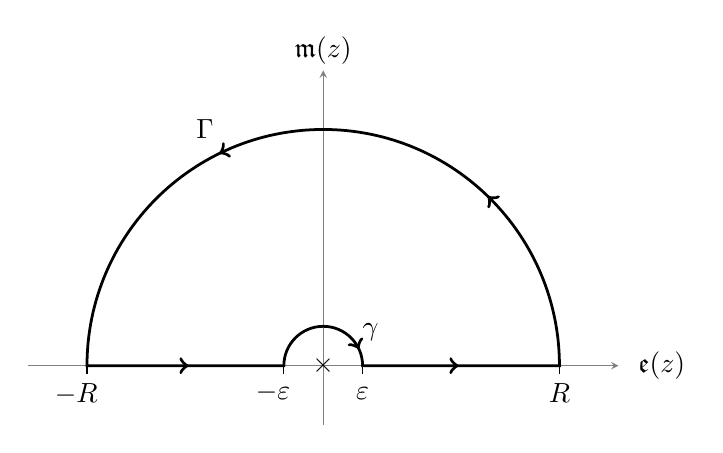
\begin{tikzpicture}
            % Configurable parameters
            \def\bigradius{3}
            \def\littleradius{0.5}

            % Axes
            \draw [help lines,-stealth] (-1.25*\bigradius, 0) -- (1.25*\bigradius,0);
            \draw [help lines,-stealth] (0, -0.25*\bigradius) -- (0, 1.25*\bigradius);
            % Red path
            \draw[line width=1pt,   decoration={ markings,
                        mark=at position 0.15 with {\arrow[line width=1.2pt]{to}},
                        mark=at position 0.38 with {\arrow[line width=1.2pt]{to}},
                        mark=at position 0.67 with {\arrow[line width=1.2pt]{to}},
                        mark=at position 0.83 with {\arrow[line width=1.2pt]{to}},
                        mark=at position 0.92 with {\arrow[line width=1.2pt]{to}}},
                postaction={decorate}]
            (0:\bigradius) arc (0:180:\bigradius)
            -- (0:-\littleradius) arc (180:0:\littleradius)
            -- cycle;
            % The labels
            \node at (4.3,0){$\Re(z)$};
            \node at (0,4) {$\Im(z)$};
            \node at (0.6,0.43) {$\gamma$};
            \node at (-1.5,3.0) {$\Gamma$};

            % The poles
            \node at (0,0) {$\times$};

            % Marks on the real axis
            \draw (-\bigradius,0) -- ++(0,-0.1) node[below] {$-R\phantom{-}$};
            \draw (-\littleradius,0) -- ++(0,-0.1) node[below] {$-\varepsilon\phantom{-}$};
            \draw (\littleradius,0) -- ++(0,-0.1) node[below] {$\vphantom{-}\varepsilon$};
            \draw (\bigradius,0) -- ++(0,-0.1) node[below] {$\vphantom{-}R$};
        \end{tikzpicture}}
    \captionsetup{justification=centering}
    \caption{The complex contour $C$}
    \label{fig:fig2}
\end{figure}

$f(z)$ is holomorphic inside $C$.
Therefore, by Cauchy's theorem,
\begin{equation*}
    \oint_{C} f(z) \diff z = 0.
\end{equation*}
Additionally, we can split this contour integral into four parts.
\begin{equation*}
    \oint_{C} f(z) \diff z = \int_{\Gamma} f(z) \diff z + \int_{-R}^{-\varepsilon} f(x) \diff x + \int_{\gamma} f(z) \diff z + \int_{\varepsilon}^{R} f(x) \diff x = 0
\end{equation*}
Consider the the second and fourth integrals.
\begin{align*}
    \int_{\varepsilon}^{R} f(x) \diff x + \int_{-R}^{-\varepsilon} f(x) \diff x & = \int_{\varepsilon}^{R} \frac{e^{ix}}{x} \diff x + \int_{-R}^{-\varepsilon} \frac{e^{ix}}{x} \diff x         \\
                                                                                & = \int_{\varepsilon}^{R} \frac{e^{ix}}{x} \diff x + \int_{R}^{\varepsilon} \frac{e^{-ix}}{-x} \cdot - \diff x \\
                                                                                & = \int_{\varepsilon}^{R} \frac{e^{ix}}{x} \diff x - \int_{\varepsilon}^{R} \frac{e^{-ix}}{x} \diff x          \\
                                                                                & = \int_{\varepsilon}^{R} \frac{e^{ix} - e^{-ix}}{x} \diff x                                                   \\
                                                                                & = 2i \int_{\varepsilon}^{R} \frac{ \sin x}{x} \diff x
\end{align*}
Notice that in the limit as $R \to \infty$ and $\varepsilon \to 0$,
\begin{align*}
    \lim_{\substack{R \to \infty                             \\ \varepsilon \to 0}} \left( \int_{\varepsilon}^{R} f(x) \diff x + \int_{-R}^{-\varepsilon} f(x) \diff x \right)  &= 2i \lim_{\substack{R \to \infty \\ \varepsilon \to 0}} \int_{\varepsilon}^{R} \frac{\sin x}{x} \diff x \\
     & = 2i \int_{0}^{\infty} \frac{\sin x}{x} \diff x       \\
     & = i \int_{-\infty}^{\infty} \frac{\sin x}{x} \diff x.
\end{align*}
We can parameterise the contour $\gamma$ by $z(t) \coloneq -\varepsilon e^{-it}$ with $t \in [0, \pi]$.
Then,
\begin{equation*}
    z'(t) = i \varepsilon e^{-it} = -i z(t).
\end{equation*}
Thus, the contour integral over $\gamma$ becomes
\begin{align*}
    \int_{\gamma} f(z) \diff z & = \int_{\gamma} \frac{e^{iz}}{z} \diff z                     \\
                               & = \int_{0}^{\pi} \frac{e^{iz(t)}}{z(t)} z'(t) \diff t        \\
                               & = \int_{0}^{\pi} \frac{e^{iz(t)}}{z(t)} \cdot -iz(t) \diff t \\
                               & = -i \int_{0}^{\pi} e^{iz(t)} \diff t                        \\
                               & = -i \int_{0}^{\pi} e^{-i\varepsilon e^{-it}} \diff t.       \\
\end{align*}
We want to take the limit of this as $\varepsilon \to 0$.
\begin{align*}
    \lim_{\varepsilon \to 0} \int_{\gamma} f(z) \diff z & = -i \lim_{\varepsilon \to 0} \int_{0}^{\pi} e^{-i\varepsilon e^{-it}} \diff t \\
                                                        & = -i \int_{0}^{\pi} \lim_{\varepsilon \to 0} e^{-i\varepsilon e^{-it}} \diff t \\
                                                        & = -i \int_{0}^{\pi} \diff t                                                    \\
                                                        & = -i \pi
\end{align*}
We interchanged the limit and integral above, which we will justify.
\begin{proposition}
    \begin{equation*}
        \lim_{\varepsilon \to 0} \int_{0}^{\pi} e^{-i\varepsilon e^{-it}} \diff t = \int_{0}^{\pi} \lim_{\varepsilon \to 0} e^{-i\varepsilon e^{-it}} \diff t
    \end{equation*}
\end{proposition}
\begin{proof}
    Let $(z_n)$ be the sequence of functions where
    \begin{equation*}
        z_{\varepsilon_n}(t) \coloneq e^{-i\varepsilon_n e^{-it}}
    \end{equation*}
    for $t \in [0, \pi]$,
    and $(\varepsilon_n) \to 0$ is arbitrary.
    We wish to shown that this sequence is uniformly bounded.
    Consider the following.
    \begin{align*}
        |z_n(t)| & = \left|e^{-i\varepsilon_n e^{-it}}\right|                                        \\
                 & = \left|e^{-i\varepsilon_n (\cos t - i\sin t)}\right|                             \\
                 & = \left|e^{-i\varepsilon_n \cos t} e^{-\varepsilon_n \sin t}\right|               \\
                 & = \left|e^{-i\varepsilon_n \cos t}\right|  \left|e^{-\varepsilon_n \sin t}\right| \\
                 & = e^{-\varepsilon_n \sin t}                                                       \\
                 & \leq e^{\varepsilon_n}
    \end{align*}
    Let $\max \{\varepsilon_n\} = 1$.
    Then,
    \begin{equation*}
        |z_n(t)| \leq e
    \end{equation*}
    for all $t \in [0, \pi]$ and for all $n \in \mathbb{N}$.
    This shows that $(z_n)$ is uniformly bounded.
    We also know that $(z_n)$ converges pointwise to $1$ for all $t \in [0, \pi]$.
    Therefore, by the bounded convergence theorem,
    \begin{equation*}
        \lim_{\varepsilon \to 0} \int_{0}^{\pi} e^{-i\varepsilon e^{-it}} \diff t = \int_{0}^{\pi} \lim_{\varepsilon \to 0} e^{-i\varepsilon e^{-it}} \diff t.
    \end{equation*}
\end{proof}
Finally, the integral over $\Gamma$ can be dealt with using Jordan's lemma.
We can parameterise the contour $\Gamma$ by $w(t) \coloneq Re^{it}$ with $t \in [0, \pi]$.
$f(z)$ is of the right form, so Jordan's lemma applies and hence,
\begin{align*}
    \left| \int_{\Gamma} f(z) \diff z \right| & \leq \pi \max_{t \in [0,\pi]} \left|\frac{1}{Re^{it}}\right| \\
                                              & = \frac{\pi}{R}
\end{align*}
Since,
\begin{equation*}
    \lim_{R \to \infty} \frac{\pi}{R} = 0,
\end{equation*}
we can conclude that
\begin{equation*}
    \lim_{R \to \infty} \int_{\Gamma} f(z) \diff z = 0.
\end{equation*}
Putting everything together, we have
\begin{alignat*}{3}
     &                & \lim_{\substack{R \to \infty                              \\ \varepsilon \to 0}} \oint_{C} f(z) \diff z & = 0 \\
     & \leadsto \quad & i\int_{0}^{\infty} \frac{\sin x}{x} \diff x      & = i\pi \\
     & \leadsto \quad & \int_{-\infty}^{\infty} \frac{\sin x}{x} \diff x & = \pi.
\end{alignat*}

\section{Dirichlet Kernel}

\begin{definition}[Dirichlet Kernel]
    The Dirichlet kernel of order $n$, $\mathcal{D}_n: \mathbb{R} \to \mathbb{R}$, is defined by
    \begin{equation}
        \mathcal{D}_n(x) \coloneq \sum_{k = -n}^{n} e^{ikx},
    \end{equation}
    where $n \in \mathbb{Z}_{\geq 0}$.
    The sequence $(\mathcal{D}_n)$ of may also be referred to as the Dirchlet kernel.
\end{definition}
\begin{proposition} \label{thm:Dirichlet kernel proposition 1}
    \begin{equation*}
        \mathcal{D}_n(x) \coloneq \sum_{k = -n}^{n} e^{ikx} = \frac{\sin\left(\left(n + \frac{1}{2}\right)x\right)}{\sin\left(\frac{x}{2}\right)}
    \end{equation*}
\end{proposition}
\begin{proof}
    Consider the geometric series
    \begin{equation*}
        \sum_{k = 0}^{n} ar^k = \frac{a(1 - r^{n+1})}{1 - r}.
    \end{equation*}
    Therefore,
    \begin{align*}
        \sum_{k=-n}^{n} r^k & = \sum_{k=0}^{n} r^k + \sum_{k=-n}^{-1} r^k                                        \\
                            & = \sum_{k=0}^{n} r^k + \sum_{k=1}^{n} r^{-k}                                       \\
                            & = \sum_{k=0}^{n} r^k + \sum_{k=0}^{n} r^{-k} - 1                                   \\
                            & = \frac{1 - r^{n+1}}{1 - r} + \frac{1 - r^{-n - 1}}{1 - r^{-1}} - 1                \\
                            & = \frac{1 - r^{n+1}}{1 - r} + \frac{r^{-n} - r}{1 - r} + \frac{r-1}{1-r}           \\
                            & = \frac{r^{-n} - r^{n+1}}{1-r}                                                     \\
                            & = \frac{r^{-n} - r^{n+1}}{1-r} \cdot \frac{r^{-\frac{1}{2}}}{r^{-\frac{1}{2}}}     \\
                            & = \frac{r^{-n-\frac{1}{2}} - r^{n+\frac{1}{2}}}{r^{-\frac{1}{2}}-r^{\frac{1}{2}}}.
    \end{align*}
    Our target sum is given by setting $r = e^{ix}$.
    \begin{align*}
        \mathcal{D}_n(x) & \coloneq \sum_{k = -n}^{n} e^{ikx}                                                                                           \\
                         & \phantom{:}= \frac{e^{-\left(n-\frac{1}{2}\right)ix} - e^{\left(n+\frac{1}{2}\right)ix}}{e^{-\frac{ix}{2}}-e^{\frac{ix}{2}}} \\
                         & \phantom{:}= \frac{-2i\sin\left(\left(n + \frac{1}{2}\right)x\right)}{-2i\sin\left(\frac{x}{2}\right)}                       \\
                         & \phantom{:}= \frac{\sin\left(\left(n + \frac{1}{2}\right)x\right)}{\sin\left(\frac{x}{2}\right)}
    \end{align*}
\end{proof}
\begin{proposition} \label{thm:Dirichlet kernel proposition 2}
    \begin{equation*}
        \mathcal{D}_n(x) \coloneq \sum_{k = -n}^{n} e^{ikx} = 1 + 2\sum_{k=1}^{n} \cos(kx)
    \end{equation*}
\end{proposition}
\begin{proof}
    \begin{align*}
        \sum_{k = -n}^{n} e^{ikx} & = 1 + \sum_{k = -n}^{-1} e^{ikx} + \sum_{k = 1}^{n} e^{ikx} \\
                                  & = 1 - \sum_{k = 1}^{n} e^{-ikx} + \sum_{k = 1}^{n} e^{ikx}  \\
                                  & = 1 + \sum_{k = 1}^{n} \left(e^{ikx} - e^{-ikx}\right)      \\
                                  & = 1 + 2\sum_{k=1}^{n} \cos(kx)
    \end{align*}
\end{proof}
The forms of the Dirichlet kernel given in Proposition~\ref{thm:Dirichlet kernel proposition 1} and Proposition~\ref{thm:Dirichlet kernel proposition 2} are more useful than its original definition for our purposes.
Integrating $\mathcal{D}$ over $[0, \pi]$ yields the following:
\begin{align*}
    \int_{0}^{\pi} \mathcal{D}_n (x) \diff x & = \int_{0}^{\pi} \left( 1 + 2\sum_{k = 1}^{n} \cos(kx) \right) \diff x       \\
                                             & = \pi + 2 \int_{0}^{\pi} \sum_{k = 1}^{n} \cos(kx)  \diff x                  \\
                                             & = \pi + 2 \sum_{k = 1}^{n} \int_{0}^{\pi} \cos(kx)    \diff x                \\
                                             & = \pi + 2 \sum_{k = 1}^{n} \left. \frac{1}{k} \sin(kx) \right|_{x=0}^{x=\pi} \\
                                             & = \pi + 2 \sum_{k = 1}^{n} 0                                                 \\
                                             & = \pi.
\end{align*}
We will use this result to evaluate the Dirichlet integral, but first, we need the Riemann-Lebesgue lemma.
\begin{lemma}[Riemann-Lebesgue Lemma] \label{thm:Riemann-Lebesgue lemma}
    Suppose $f: \mathbb{R} \to \mathbb{R}$ is Lebesgue integrable on $[a,b] \subset \mathbb{R}$.
    Then,
    \begin{equation} \label{eq:Riemann-Lebesgue lemma equation}
        \lim_{\lambda \to \infty} \int_{a}^{b} f(x) e^{i\lambda x} \diff x = 0.
    \end{equation}
\end{lemma}
\begin{corollary} \label{thm:Riemann-Lebesgue corollary}
    \begin{equation}
        \lim_{\lambda \to \infty} \int_{a}^{b} f(x) \cos(\lambda x) \diff x = 0
    \end{equation}
    and
    \begin{equation}
        \lim_{\lambda \to \infty} \int_{a}^{b} f(x) \sin(\lambda x) \diff x = 0.
    \end{equation}
\end{corollary}
\begin{proof}
    By the fact that $f$ is real-valued via assumption, one can take the real and imaginary parts of Equation~\eqref{eq:Riemann-Lebesgue lemma equation} to obtain the desired results:
    \begin{alignat*}{3}
         &                & \Re \left(\lim_{\lambda \to \infty} \int_{a}^{b} f(x) e^{i\lambda x} \diff x \right) & = 0  \\
         & \leadsto \quad & \lim_{\lambda \to \infty} \Re \left(\int_{a}^{b} f(x) e^{i\lambda x} \diff x \right) & = 0  \\
         & \leadsto \quad & \lim_{\lambda \to \infty} \int_{a}^{b} \Re\left( f(x) e^{i\lambda x}\right) \diff x  & = 0  \\
         & \leadsto \quad & \lim_{\lambda \to \infty} \int_{a}^{b} f(x) \Re\left( e^{i\lambda x}\right) \diff x  & = 0  \\
         & \leadsto \quad & \lim_{\lambda \to \infty} \int_{a}^{b} f(x) \cos(\lambda x) \diff x                  & = 0,
    \end{alignat*}
    and similarly,
    \begin{alignat*}{3}
         &                & \Im \left(\lim_{\lambda \to \infty} \int_{a}^{b} f(x) e^{i\lambda x} \diff x \right) & = 0  \\
         & \leadsto \quad & \lim_{\lambda \to \infty} \int_{a}^{b} f(x) \Im\left( e^{i\lambda x}\right) \diff x  & = 0  \\
         & \leadsto \quad & \lim_{\lambda \to \infty} \int_{a}^{b} f(x) \sin(\lambda x) \diff x                  & = 0.
    \end{alignat*}
\end{proof}
Define $f: \mathbb{R} \setminus \{n \in \mathbb{R} \mid n = 2\pi k, \; k \in \mathbb{Z} \} \to \mathbb{R}$ by
\begin{equation*}
    f(x) \coloneq \frac{1}{\sin\left(\frac{x}{2}\right)} - \frac{2}{x}.
\end{equation*}
Since $f$ is Lebesgue integrable on $[0, \pi]$, Corollary~\ref{thm:Riemann-Lebesgue corollary} of the Riemann-Lebesgue lemma allows us to state that
\begin{alignat*}{3}
     &                & \lim_{\lambda \to \infty} \int_{0}^{\pi} \left(\frac{1}{\sin\left(\frac{x}{2}\right)} - \frac{2}{x}\right) \sin(\lambda x) \diff x                                                                                                                    & = 0              \\
     & \leadsto \quad & \lim_{\lambda \to \infty} \int_{0}^{\pi} \left(\frac{1}{\sin\left(\frac{x}{2}\right)} - \frac{2}{x}\right) \sin\left(\left(\lambda  + \frac{1}{2}\right)x\right) \diff x                                                                              & = 0              \\
     & \leadsto \quad & \lim_{\lambda \to \infty} \left( \int_{0}^{\pi} \frac{\sin\left(\left(\lambda  + \frac{1}{2}\right)x\right)}{\sin\left(\frac{x}{2}\right)} \diff x - 2 \int_{0}^{\pi} \frac{\sin\left(\left(\lambda  + \frac{1}{2}\right)x\right)}{x} \diff x \right) & = 0              \\
     & \leadsto \quad & \lim_{\lambda \to \infty} \left( \int_{0}^{\pi} \mathcal{D}_n(x) \diff x - 2 \int_{0}^{\pi} \frac{\sin\left(\left(\lambda  + \frac{1}{2}\right)x\right)}{x} \diff x \right)                                                                           & = 0              \\
     & \leadsto \quad & \lim_{\lambda \to \infty} \left( \pi - 2 \int_{0}^{\pi} \frac{\sin\left(\left(\lambda  + \frac{1}{2}\right)x\right)}{x} \diff x \right)                                                                                                               & = 0              \\
     & \leadsto \quad & \pi - 2 \lim_{\lambda \to \infty} \int_{0}^{\pi} \frac{\sin\left(\left(\lambda  + \frac{1}{2}\right)x\right)}{x} \diff x                                                                                                                              & = 0              \\
     & \leadsto \quad & \lim_{\lambda \to \infty} \int_{0}^{\pi} \frac{\sin\left(\left(\lambda  + \frac{1}{2}\right)x\right)}{x} \diff x                                                                                                                                      & = \frac{\pi}{2}.
\end{alignat*}
By changing variables, we get
\begin{alignat*}{3}
     &                & \lim_{\lambda \to \infty} \int_{0}^{\left(\lambda  + \frac{1}{2}\right) \pi} \frac{\sin x}{x} \diff x  = \frac{\pi}{2}                                                                             \\
     & \leadsto \quad & \lim_{\lambda \to \infty} \int_{0}^{\left(\lambda  + \frac{1}{2}\right) \pi} \frac{\sin x}{x} \diff x                                                                           & = \frac{\pi}{2}  \\
     & \leadsto \quad & \lim_{\lambda \to \infty} \left(\int_{0}^{\lambda \pi} \frac{\sin x}{x} \diff x + \int_{\lambda \pi}^{\left(\lambda  + \frac{1}{2}\right) \pi} \frac{\sin x}{x} \diff x \right) & = \frac{\pi}{2}.
\end{alignat*}
From the proof of Proposition~\ref{thm:convergence proposition 1}, we know that
\begin{equation*}
    \int_{0}^{\infty} \frac{\sin x}{x} \diff x \coloneq \lim_{\lambda \to \infty} \int_{0}^{\lambda} \frac{\sin x}{x} \diff x = \lim_{\lambda \to \infty} \int_{0}^{\lambda \pi} \frac{\sin x}{x} \diff x.
\end{equation*}
Additionally, as $\lambda \to \infty$,
\begin{align*}
    \left|\int_{\lambda \pi}^{\left(\lambda  + \frac{1}{2}\right) \pi} \frac{\sin x}{x} \diff x \right| & \leq \int_{\lambda \pi}^{\left(\lambda  + \frac{1}{2}\right) \pi} \frac{|\sin x|}{x} \diff x \\
                                                                                                        & \leq \int_{\lambda \pi}^{\left(\lambda  + \frac{1}{2}\right) \pi} \frac{\diff x}{x}          \\
                                                                                                        & = \ln \left(\frac{\left(\lambda  + \frac{1}{2}\right) \pi}{\lambda \pi}\right) \to 0         \\
    \leadsto \quad                                                                                      & \int_{\lambda \pi}^{\left(\lambda  + \frac{1}{2}\right) \pi} \frac{\sin x}{x} \diff x \to 0.
\end{align*}
Hence,
\begin{equation*}
    \lim_{\lambda \to \infty} \int_{0}^{\lambda \pi} \frac{\sin x}{x} \diff x + \lim_{\lambda \to \infty} \int_{\lambda \pi}^{\left(\lambda  + \frac{1}{2}\right) \pi} \frac{\sin x}{x} \diff x = \frac{\pi}{2}
\end{equation*}
gives
\begin{equation*}
    \int_{0}^{\infty} \frac{\sin x}{x} \diff x = \frac{\pi}{2},
\end{equation*}
so
\begin{equation*}
    \int_{-\infty}^{\infty} \frac{\sin x}{x} \diff x = \pi.
\end{equation*}

\section{Fourier Transform}

\begin{definition}[Fourier Transform]
    Let $f: \mathbb{R} \to \mathbb{R}$ be Lebesgue integrable.
    The Fourier transform of $f$, denoted $\mathscr{F}\{f\}$, is a function of $s \in \mathbb{R}$ defined by
    \begin{equation}
        \mathscr{F}\{f\} (\omega) \coloneq \int_{-\infty}^{\infty} e^{-2i\pi \omega t} f(t) \diff t.
    \end{equation}
\end{definition}
\begin{theorem}[Fourier Inversion Theorem] \label{thm:Fourier inversion theorem}
    Let $f: \mathbb{R} \to \mathbb{R}$ be Lebesgue integrable and piecewise smooth.
    Define the inverse Fourier transform of $\mathscr{F}\{f\}$, denoted $\mathscr{F}^{-1}\{\mathscr{F}\{f\}\}$, as
    \begin{equation}
        \mathscr{F}^{-1}\{\mathscr{F}\{f(t)\}(\omega)\}(t) \coloneq \int_{-\infty}^{\infty} \mathscr{F}\{f(t)\}(\omega) e^{2i\pi\omega t} d\omega.
    \end{equation}
    Then,
    \begin{equation*}
        f(t) = \mathscr{F}^{-1}\{\mathscr{F}\{f(t)\}(\omega)\}(t)
    \end{equation*}
    for all $t \in \mathbb{R}$.
\end{theorem}
Let $f: \mathbb{R} \to \mathbb{R}$ be defined by
\begin{equation*}
    f(t) \coloneq
    \begin{cases}
        1 & \text{if } |t| < 1, \\
        0 & \text{otherwise}.
    \end{cases}
\end{equation*}
$f$ is Lebesgue integrable and piecewise smooth, and its Fourier transform is
\begin{align*}
    \mathscr{F}\{f(t)\}(\omega) & = \int_{-\infty}^{\infty} e^{-2i\pi \omega t} f(t) \diff t                \\
                                & = \int_{-1}^{1} e^{-2i\pi \omega t} \diff t                               \\
                                & = \left. - \frac{1}{2i\pi\omega} e^{-2i\pi \omega t} \right|_{t=-1}^{t=1} \\
                                & = -\frac{e^{-2i\pi \omega} - e^{2i\pi \omega}}{2i\pi\omega}               \\
                                & = \frac{e^{2i\pi \omega} - e^{-2i\pi \omega}}{2i\pi\omega}                \\
                                & = \frac{\sin(2\pi \omega)}{\pi\omega}.
\end{align*}
By Theorem~\ref{thm:Fourier inversion theorem},
\begin{equation*}
    f(t) = \int_{-\infty}^{\infty} \frac{\sin(2\pi \omega)}{\pi\omega} e^{2i\pi\omega t} d\omega = \frac{1}{\pi} \int_{-\infty}^{\infty} \frac{\sin \omega}{\omega} e^{i\omega t} d\omega.
\end{equation*}
At $t=0$:
\begin{equation*}
    f(0) = 1 = \frac{1}{\pi} \int_{-\infty}^{\infty} \frac{\sin \omega}{\omega} d\omega.
\end{equation*}
Therefore,
\begin{equation*}
    \int_{-\infty}^{\infty} \frac{\sin \omega}{\omega} d\omega = \pi.
\end{equation*}

\end{document}